\documentclass[10pt, a4paper]{article}

\usepackage[utf8]{inputenc}
\usepackage[portuges]{babel}
\usepackage{blindtext}
\usepackage{enumitem}
\usepackage{graphicx}
\usepackage{cite}

\title{Desenvolvimento de Sistemas de Software \\ \large{Mestrado Integrado em Engenharia Informática}}
\author{Luís Capa \\ A81960 \\ 
\includegraphics[width = 20mm]{luis}
	\and 
	Moisés Antunes \\ A82263 \\ 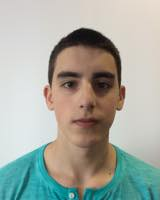
\includegraphics[width = 20mm]{moises}
	\and
	Pedro Capa \\ A83170 \\ 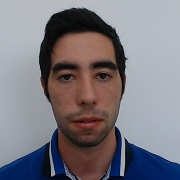
\includegraphics[width = 20mm, height = 25mm]{pedro}
}
\date{\today}

\renewcommand{\baselinestretch}{1.2}

\newpage
\begin{document}
\maketitle
\tableofcontents

\newpage
\section{Introdução}\label{Intro}
Hoje em dia, os clientes das grandes marcas de automóveis têm a possibilidade de personalizar o carro da maneira como quiserem. Para tal, os clientes podem escolher peça a peça, escolher um pacote ou escolher configuração ótima em relação ao orçamento. O cliente não pode escolher todas as peças que quer, visto que há peças que são incompatíveis e outras que são obrigatórias. Os componentes na fábrica têm um stock, no caso de chegarem novas peças é necessário informar o sistema que chegaram novas peças e os carros que estão à espera dessas peças voltam para a fila de produção.
Como este modelo de compra está a ser muito usado, o trabalho de DSS deste ano consistia em modelar o problema, recorrendo à linguagem de modelação UML, para criar a interface gráfica da aplicação e para criar as classes deste projeto, foi recorrido à linguagem de programação Java.

\section{Objetivos}\label{objetivos}
Esta unidade curricular tem o objetivo de mudar a forma como nós programamos, pois até agora sempre que recebiamos um projeto o primeiro pensamento era escrever código. Para isso usou-se a linguagem UML para preparar a escrita do código de forma a cometer menos erros quer na criação de classes e nas suas variáveis de instância quer ter uma representação gráfica do sistema a ser desenvolvido.
Este relatório tem o objetivo de clarificar o trabalho realizado no geral, bem como as suas partes.

\newpage
\section{Trabalho realizado}\label{trabalho}
Para este trabalho foram criados alguns modelos UML como o modelo de dominio, UseCase, os diagramas de estado, os diagramas de sequência, diagramas de classes e os diagramas de packages.
\subsection{Modelo de domínio}
Inicialmente, no "Visual Paradigm" foi criado um modelo de domínio que mostra as prinicipais relações entre entidades criadas para este problema, a título de exemplo, foram consideradas algumas relações entre os componentes do carro.
\subsection{Diagrama de use cases}
De seguida, no mesmo programa foi criado o modelo de use cases. Este modelo mostra as principais interações entre os atores do sistema com o própio sistema.De notar que só foram criados os use cases que achamos absolutamente necessário para cumprir alguns requisitos pré-estabelecidos. Para cada use case foi feita uma descrição detalhada da iteração entre o ator e o sistema. Neste sistema foram considerados dois atores, o cliente que faria a compra online e o funcionário que utilizaria a aplicação na fábrica.

O cliente tem os seguintes use cases:
\begin{itemize}
\item Registar;
\item Comprar carro;
\item Ver lista de carros comprados;
\item Escolher pacote;
\item Escolher especificações;
\item Escolher configuração ótima;
\item Login
\end{itemize}
O Funcionário tem os seguintes use cases:
\begin{itemize}
\item Login
\item Adicionar stock
\item Ver stock disponível
\item Carro pronto
\item Ver lista de carros
\end{itemize}

\subsection{Máquinas de estado}
No desenvolvimento da aplicação foram consideradas duas entidades que teriam diferentes estados, o carro e a peça. Para descrever as diferentes fases destas entidades foi criado para cada uma um modelo de estado.

Para o carro foram considerados os seguintes estados:
\begin{description}[align=left]
\item [Em espera] Quando algum componente do carro está sem stock;
\item [Em produção] No caso de todos os componentes para o carro existirem;
\item [Pronto] Ao fim do carro ser produzido;
\end{description}

A peça ou componente tinham os seguintes estados:
\begin{description}[align=left]
\item [Esgotado] Se não houver em stock esta peça;
\item [Disponível] No caso de haver em stock esta peça
\end{description}
\subsection{Diagrama de sequência de sistema}
Para se obter uma melhor perceção da interação entre o cliente e o sistema foram criados os DSS para cada use case. Inicialmente foram usadas as descrições dos use cases criados em "Excel", para criar um modelo simples, mas em seguida foram criados mais alguns DSS e em cada um era aumentado o detalhe. Em segundo lugar, foram criados os DSS que além de representar a interação do sistema com o utilizador, também representava a relação entre a interface do sistema e a camada de negócio deste. Em sguida foram criados os DSS de subsistemas, que, basicamente, representa as várias entidades no sistema e como cada use case interage com essas entidades, por exemplo o use case "Adicionar Stock" relacionava-se com o subsistema da peça e do carro. De seguida, foram criados DSS para especificar os métodos que eram utilizados nos DSS anteriores. A partir de alguns dos útlimos DSS, aqueles que tinham de aceder à base de dados, foram criados uns DSS, em que as listas e os conjuntos de entidades eram subsitituídas por DAO, classes que acediam à base de dados, por exemplo no método getListaCarrosComprados(), antes o sistema ia a um map buscar os carros que eram do cliente, mas no último DSS esse map era substituído pela classe CarroDAO, que continha um método para trazer da base de dados as especificações dos carros que o cliente comprou.
\subsection{Diagrama de classes}
Para os DSS criados foi criado um diagrama de classes, que indicava as classes que eram precisas criar, as variáveis de instância para cada classe e todos os métodos que eram necessários implementar. Não foram criados diagramas de classes para todos os DSS, pois os use cases do "Escolher configuração ótima", "Escolher Especificações" e o "Escolher Pacote" foram todos incluídos no diagrama de classes do "Comprar Carro", pois os métodos nestes DSS eram quase sempre os mesmos e achamos que não havia necessidade de criar diagramas de classes para cada um. O mesmo aconteceu para os diagramas de classes para os DSS que tinham os DAO.
No fim de todos os diagramas de classes serem feitos, foram todos juntados num só, em que continha todas as classes, variáveis de instância e métodos.
\subsection{Diagrama de packages}
Em seguida, os diagramas de classes e o modelo de domínio foram divididos em packages. Além destes diagramas de packages, do mesmo modo foi criado um diagrama de packages para demonstrar as diferentes camadas aplicacionais do sistema. Esta foi dividida em três partes, a Interface, a camada de negócio e a base de dados. Na camada de negócio estava contida as várias classes do sistema.
\subsection{Codificação da aplicação}
Finalmente, foi começado a implementar a aplicação, na qual o trabalho foi dividido em três partes, a interface, a base de dados e a camada de negócio. Cada uma destas partes foi feita por cada um dos elementos do grupo. No entanto, quando foram criadas as classes DAO foi notado que na altura de carregar os dados, por exemplo de uma peça podia ser carregado para memória muitas peças que nem eram precisas, uma vez que uma peça tem uma lista de peças proibidas e uma lista de peças obrigatórias, ou seja para carregar uma peça da base de dados tinha-se de levar por arrasto muitas peças. Este problema também se verificava com os carros, por causa da lista de peças que um carro tem. Depois deste problema foi dicidido alterar algumas classes, que continham listas, como por exemplo a peça em vez de ter uma lista de peças passou a ter uma lista de string.

A interface foi criada no "NetBeans", uma vez que é mais fácil de implementar a interface gráfica, porque tem um visualisador de classes de interfaces e gera automaticamente o código dos componentes do swing, api de interfaces usada. A interface foi modelada de acordo com os Use Cases do projeto, uma vez que este indica que opções cada ator realiza no sistema.

A base de dados utilizada foi  "MySQL", porque já tinha sido explorada em outras UC, mas também por ser uma base de dados relacional.

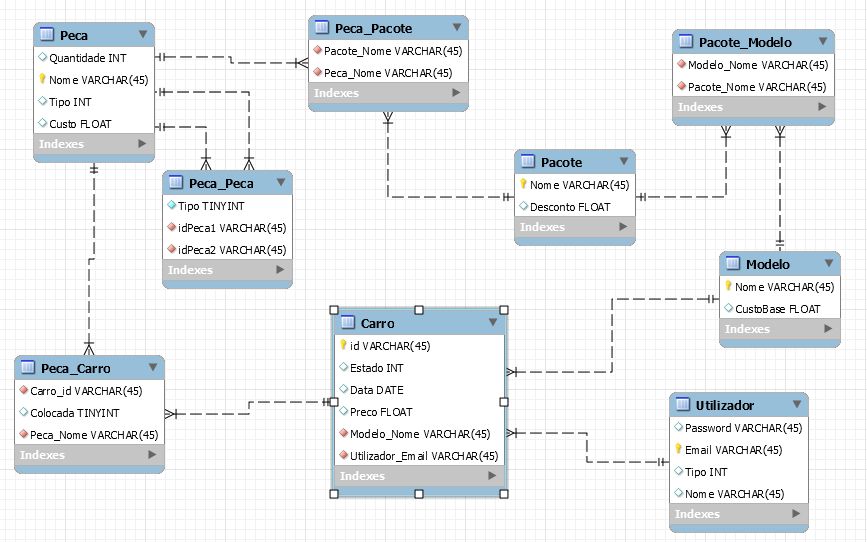
\includegraphics{EsquemaFisico}

As classes criadas e que estavam representadas nos diagramas de classes foram as seguintes:
\begin{itemize}
\item ConfiguraFacil
\item Carro
\item Utilizador
\item Funcionario - Subclasse de Utilizador
\item Cliente - Subclasse de Utilizador
\item Peca
\item Extra - Subclasse de Peca
\item Motor - Subclasse de Peca
\item Jantes - Subclasse de Peca
\item Cor - Subclasse de Peca
\item Estofos - Subclasse de Peca
\item Modelo
\item Pacote
\end{itemize}

O carro tem duas listas de string, em que uma indica as peças que já foram colocadas no carro e a outra mostra as peças que faltam colocar no carro. O carro tem o email do utilizador que o comprou, uma vez que era mais fácil de guardar os dados na base de dados se cada carro tivesse o email do comprador e um utilizador tem uma lista de id dos carros que comprou, porque se o utilizador quisesse ver a lista de carros que tinha comprado era muito mais rápido.

Por fim, a base de dados foi povoada e foram feitos alguns testes, que foi útil para corrigir pequenos erros no código.

\section{Funcionamento da aplicação}

Como já foi referido acima há dois tipos de utilizadores, os clientes e os funcionários. Os funcionários são responsáveis por colocar um carro em produção pronto e adicionar peças na fábrica. Quando são adicionadas peças pelos funcionários, o sistema verifica se há algum carro à espera dessa peça e põe essa peça como colocada no carro. O cliente tem acesso à lista de carros que comprou, pode comprar um carro de três formas diferentes, escolher um pacote, escolher a melhor configuração com um determinado orçamento ou personalizar por completo o carro. Na compra do carro, o cliente escolhe primeiro qual o modelo do carro e só em seguida escolhe a forma de compra. Se um cliente escolher um pacote, este não tem a opção de alterar as peças obrigatórias, neste caso, o motor, a cor, jantes e estofos, no entanto, pode escolher todas os extras que quiser. Ao escolher esta opção o cliente tem um desconto associado a cada pacote. Se o cliente escolher personalizar tem a possiblidade de escolher todas as peças que quiser, desde que não tenha peças incompatíveis ou não tenha peças obrigatórias em falta. Ao escolher a configuração ótima não há garantia que tenha a melhor configuração dado o orçamento disponível. Nesta opção o sistema vai tentar encontrar o melhor pacote para, ou seja, o pacote mais caro para o dado modelo e orçamento que escolheu. Se ainda houver margem o sistema vai adicionar todos os extras que puder, começando sempre por adicionar os mais caros. Este algoritmo não garante que seja escolhida a melhor configuração, pois não verifica todas as diferentes.

\newpage
\section{Análise crítica do trabalho realizado}\label{analise}
Vários “Use Cases” foram criados para garantir acesso a um sistema que permita tanto aos clientes como funcionários proceder à compra, venda e outras operações relativas aos automóveis da empresa. O nosso objetivo principal durante a criação destes “Use Cases” foi garantir que haveria várias opções de customização de carros e que os utilizadores do sistema teriam acesso aos dados que lhes diziam respeito sem, no entanto, exagerar na quantidade de opções disponíveis, que deixaria o sistema demasiado complicado de usar, especialmente para clientes não acostumados com algo do género.

Nos modelos de estado consideramos que os principais métodos e interações com as entidades foram considerados, apesar de eventualmente haver algum em falta, por exemplo não foi considerado o caso de alguma peça não ser mais produzida pelos fornecedores da fabrica.

Para o modelo de domínio acreditamos que os principais conceitos e relações entre entidades foram inseridas neste modelo.

No final, acreditamos que o trabalho que desenvolvemos até agora demonstra bem esse equilíbrio entre personalização e facilidade de uso que procuramos, que são apenas detalhes, mas é neles que se destaca uns projetos dos outros. Também achamos que o essencial foi feito apropriadamente e que não há falta de alguma funcionalidade que seja absolutamente necessário, sendo que consideramos o trabalho até agora tanto funcional como cómodo para o utilizador. Como não tinhamos muita prática em modelação, à medida que o projeto era desenvolvido verificamos que eram cometidos alguns erros na modelação, que nos obrigava a reformular alguns modelos, retardando o desenvolvimento do projeto. Foi notado que se passou menos tempo a corrigir erros no código, mas também foram criados menos métodos e que só foram criados os métodos que eram necessários no desenvolvimento do projeto, comparando com outros projetos, que por vezes eram criados métodos que nunca eram utilizados.
\end{document}